\subsection{Lists}

\begin{breakbox}

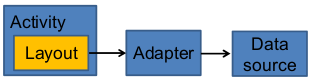
\includegraphics[width=0.15\textwidth]{figures/listBinding.png}

The List is displayed on the activity and the data is binded via an adapter. You can
also define an alternative to display, when the list is empty.

\end{breakbox}

\begin{breakbox}
\boxtitle{Code Example}

\begin{lstlisting}
protected void onCreate(Bundle savedInstanceState) {
    super.onCreate(savedInstanceState);
    setContentView(com.example. arrayadapterdemo.R.layout.main);
    loadContent(); // load content into ArrayList<String> mValues

    ArrayAdapter<String> adapter = new ArrayAdapter<String>(this, android.R.layout. simple_list_item_1, mValues);
    // this is the current context
    // simple_list_item_1 resource id for the layout of a single row
    // mValues are the objects to display

    setListAdapter(adapter); // assign adapter to ListView
}
\end{lstlisting}
\end{breakbox}


\subsection{RecyclerView}
\begin{breakbox}
RecyclerView is a more sophisticated alternative to display lists and
grids and is optimized. 
\begin{itemize}
    \item Fast scrolling through large lists/grids is an issue
    \item Items are added or removed at run-time - Item add or removal is to be animated
\end{itemize}

The RecyclerView uses the existing rows in the List and fill them with
new content while scrolling, instead of creating new elements for every
entry while scrolling (List is doing so). \\
The layout of the RecyclerView as a whole is determined by choosing a LayoutManager
e.g.\textasciitilde{}LinearLayoutManager, GridLayoutManager or
StaggeredGridLayoutManager.
\end{breakbox}

\begin{breakbox}
\boxtitle{RecyclerViewHolder}

The RecyclerViewHolder is responsible to bind the data between the model
and the adapter. The adapter there is just a dump object to do the
connection between the view and the RecyclerViewHolder. The
RecyclerViewHolder has the method bindData() which binds the data from
the model to the adapter.

\begin{lstlisting}
public class SimpleViewHolder extends RecyclerView.ViewHolder {
    private TextView simpleTextView;

    public SimpleViewHolder(final View itemView) {
        super(itemView);
        simpleTextView = (TextView) itemView.findViewById (R.id.simple_text);
    }

    public void bindData(final SimpleViewModel viewModel) {
        simpleTextView.setText (viewModel.getSimpleText());
    }
}
\end{lstlisting}
\end{breakbox}


\subsection{Fragments}

\begin{breakbox}
\begin{itemize}
    \item Fragments have their own view
layout, which can be declared in XML and defined in Java
\item This layout
can be inserted into an activity
\item Fragments have their own lifecycle

\end{itemize}

\end{breakbox}

\begin{breakbox}
\boxtitle{FragmentManager}

To change things on diffrent fragments, you have to use a fragment
transaction with the \textbf{FragmentManager}.

\begin{lstlisting}
// obtain a reference to a new fragment to show the selection details = DetailsFragment.newInstance(index);
// perform the transaction to replace any existing fragment (while the activity is in resumed lifecycle state !)
FragmentTransaction ft = getFragmentManager(). beginTransaction();
ft.replace(R.id.details, details);
ft.setTransition (FragmentTransaction. TRANSIT_FRAGMENT_FADE); // standard transition animation
// enable reverting the Fragment change via the back button
// ft.addToBackStack(null); // conserve previous old details fragment
ft.commit(); // schedule transaction
\end{lstlisting}
\end{breakbox}

\begin{breakbox}
\boxtitle{Accessing the activity within the fragment}

\begin{lstlisting}
Activity activity = getActivity();
\end{lstlisting}
\end{breakbox}

\begin{breakbox}
\boxtitle{Accessing fragments within the activity}

\begin{lstlisting}
DetailsFragment fragment = (DetailsFragment) getFragmentManager().findFragmentById (R.id.details_fragment);
\end{lstlisting}
\end{breakbox}

\begin{breakbox}
\boxtitle{Decoupling the Fragments}

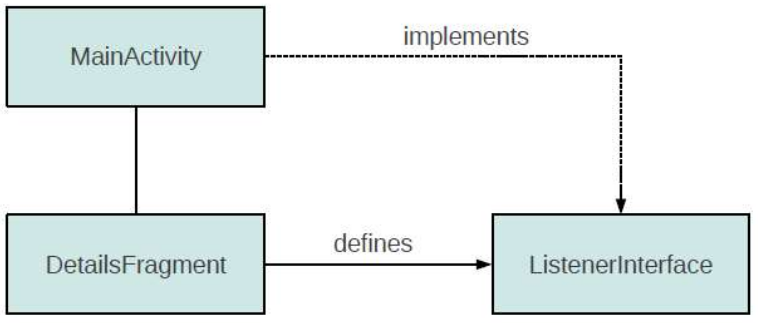
\includegraphics[width=0.24\textwidth]{figures/decouplingFragments.png}

In the Fragment Class you have an internal public interface and
the method onAttach.

\begin{lstlisting}
public class MyListFragment extends ListFragment {
    private OnItemSelectedListener listener;

    public interface OnItemSelectedListener {
        public void onRssItemSelected(String link);
    }

    public void onAttach(Activity activity) {
        super.onAttach(activity);
        listener = (OnItemSelectedListener) activity;
    }

    public void onListItemClick(ListView l, View v, int position, long id) {
        String title = l.getItemAtPosition (position).toString();
        RssItem rssItem = list.get(position);
        listener.onRssItemSelected (rssItem.getTitle());
        super.onListItemClick(l, v, position, id);
    }
\end{lstlisting}

In the Activity Class you need to implement this interface.

\begin{lstlisting}
public class RssfeedActivity extends Activity implements
    MyListFragment.OnItemSelectedListener {

    public void onRssItemSelected(String link) {
        // Find DetailsFragment in layout and update
        DetailsFragment fragment = (DetailsFragment)
        getFragmentManager(). findFragmentById (R.id.DetailsFragment);
        if (fragment != null && fragment.isInLayout()) {
            fragment.setText(link);
        } else {
            // start DetailsActivity as we are on a device with small screen
        }
    }
}
\end{lstlisting}
\end{breakbox}
